\clearpage
\section{From BPMN modelling to Petri nets}
\label{sec:models}

\begin{figure}[h]
  \centering
  \begin{tikzpicture}
    \node[anchor=south west, inner sep=0] (img) at (0,0)
      {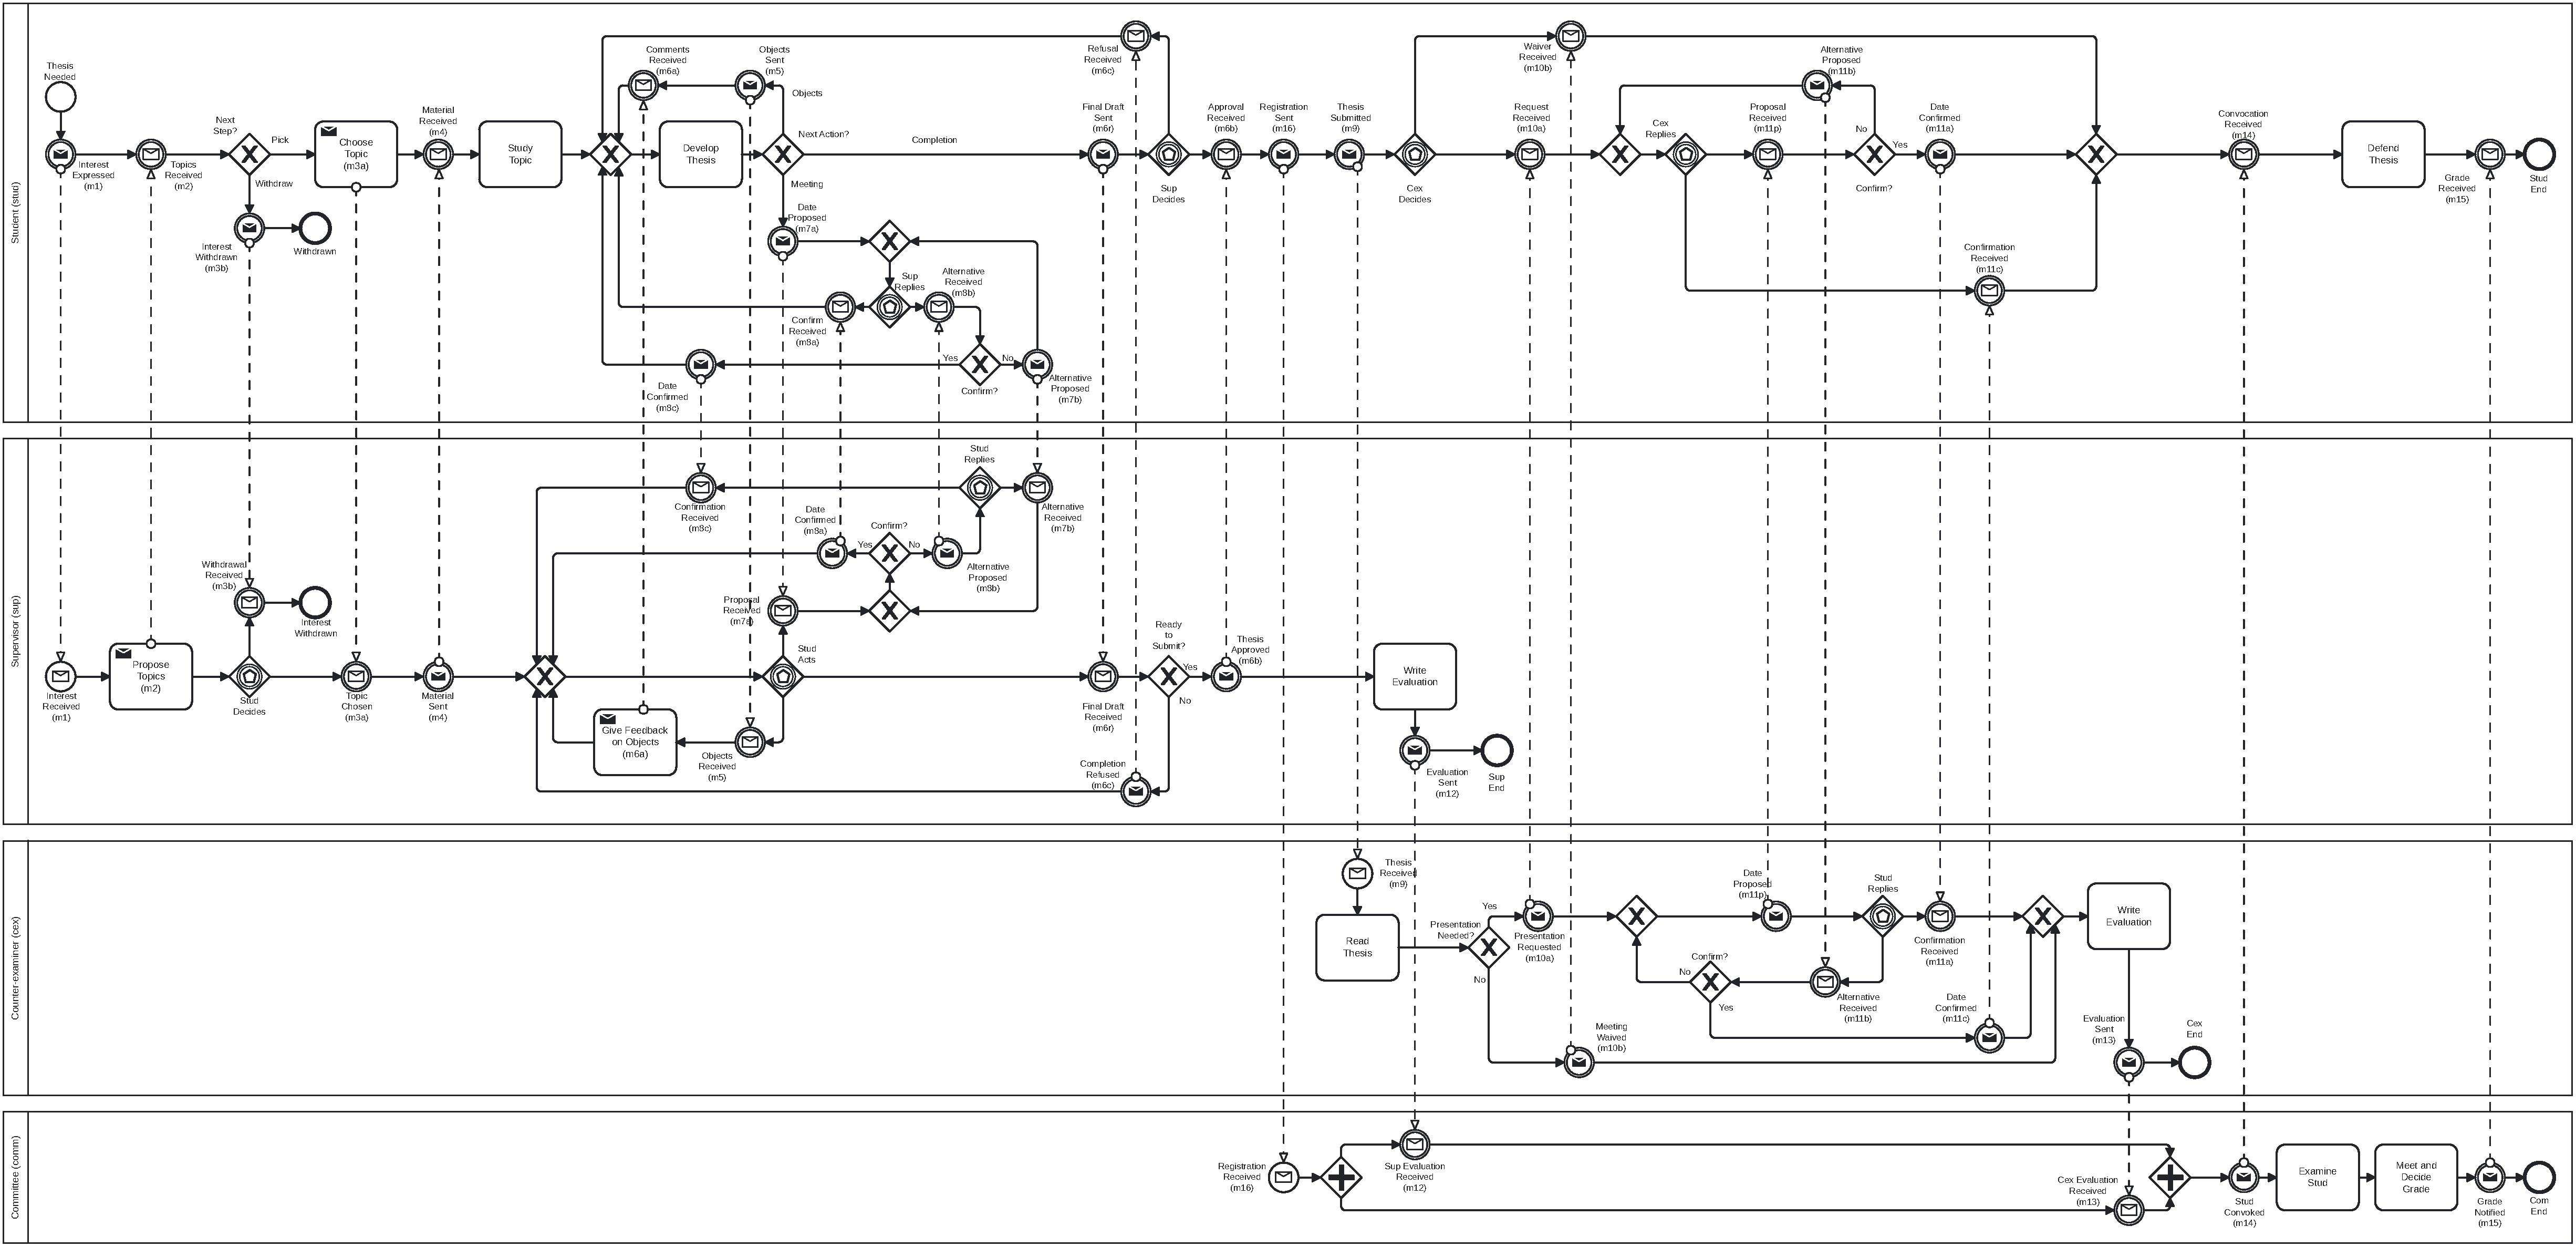
\includegraphics[width=\linewidth]{../bpmn/img/collaboration.pdf}};
    \begin{scope}[x={(img.south east)}, y={(img.north west)}]
      \foreach \bx in {0.183, 0.487, 0.860}
        \draw[dashed, thick, unipiblue] (\bx, 0) -- (\bx, 1.105);
      \foreach \bx/\lbl in {0.091/{Interest and Topic}, 0.335/{Thesis Development},
                            0.673/{Submission and Assessment}, 0.930/{Graduation}}
        \node[overlay, font=\scriptsize\bfseries, text=unipiblue] at (\bx, 1.075) {\lbl};
    \end{scope}
  \end{tikzpicture}
  \caption{The collaboration (\texttt{bpmn/collaboration.bpmn}), cut into the four phases of
    \cref{sec:collaboration}.}
  \label{fig:collaboration}
\end{figure}


\Cref{fig:collaboration} is the whole model: one row per participant, four orchestrations in all (\cref{sec:orchestrations}), running together through the four phases of the collaboration (\cref{sec:collaboration}). No wait in it carries a deadline, since we assume every participant answers in the end, so the model has no timer and no branch for an answer that never comes.

\subsection{Orchestrations}
\label{sec:orchestrations}

In each orchestration, and in the collaboration, a joint act takes a task only where the messages alone do not show it happened. When both participants send or receive the message that settles it, as with the acceptance of a meeting date, it takes none. If only one side sends, as with the convocation to the examination, nothing shows that the student attended, and the act takes a task on each side. \Cref{tab:elements} counts the elements of each orchestration.

\begin{table}[!h]
  \centering
  \vspace{2em}
  \renewcommand{\arraystretch}{1.08}
  \rowcolors{2}{}{rowshade}
  \begin{tabular}{@{}l ccccc@{}}
    \toprule
    & \textbf{Student} & \textbf{Supervisor} & \textbf{Counter-examiner} & \textbf{Committee} & \textbf{Total} \\
    \midrule
    start / end events & 1 / 2 & 1 / 2 & 1 / 1 & 1 / 1 & 4 / 6 \\
    tasks (send tasks) & 4 (1) & 3 (2) & 2 (0) & 2 (0) & 11 (3) \\
    intermediate catch events & 13 & 7 & 2 & 2 & 24 \\
    intermediate throw events & 11 & 6 & 5 & 2 & 24 \\
    event-based gateways & 4 & 3 & 1 & 0 & 8 \\
    exclusive gateways & 8 & 4 & 4 & 0 & 16 \\
    parallel gateways & 0 & 0 & 0 & 2 & 2 \\
    \midrule
    nodes & 43 & 26 & 16 & 10 & 95 \\
    sequence flows & 50 & 30 & 18 & 10 & 108 \\
    \bottomrule
  \end{tabular}
  \caption{Element counts for the four orchestrations.}
  \label{tab:elements}
\end{table}
\textbf{Student} (\texttt{bpmn/student.bpmn}). Each round of the development loop opens on \textsf{Develop Thesis} and reaches the XOR-split \textsf{Next Action?}, which offers three moves towards the supervisor: send an object, propose a meeting date, or send the final draft and ask whether the work is done. Keeping them exclusive rules out the runs where the supervisor is annotating a draft while a date is still open, and it leaves the pool an S-net.

Once the supervisor approves, the student registers for the graduation call and only then sends the thesis to the counter-examiner. The student waits to hear whether the counter-examiner wants a presentation, confirms or counters the date they propose, and ends on the convocation, \textsf{Defend Thesis} and the grade.

\textbf{Supervisor} (\texttt{bpmn/supervisor.bpmn}). The student's withdrawal closes this orchestration at once. Otherwise it mirrors the student's, with one wait for the three branches a round can take and another after the supervisor counter-proposes a date. It ends when the supervisor writes the evaluation and sends it to the committee.

\textbf{Counter-examiner} (\texttt{bpmn/counter-examiner.bpmn}). \textsf{Read Thesis} precedes the XOR-split \textsf{Presentation Needed?}. The counter-examiner either waives the meeting or asks for one and proposes a date, which the student confirms or counters until both agree. The branches merge, and \textsf{Write Evaluation} follows, so whatever the presentation settles reaches the evaluation.

\textbf{Committee} (\texttt{bpmn/committee.bpmn}). Nothing orders the supervisor's evaluation against the counter-examiner's, and the assignment makes the examination and the reading two prerequisites of the same meeting, so the orchestration waits for the two evaluations in parallel and joins before convoking the student. That is the one AND in the model.

\subsection{Collaboration}
\label{sec:collaboration}

Twenty-seven message flows wire the four pools in the collaboration (\cref{tab:messages}). The student's pool is the axis: it touches twenty-five, missing only the two evaluations that reach the committee. The student also instantiates all three of the others, one message each. Because that pool runs through all of it, the collaboration reads as four phases, drawn over \cref{fig:collaboration} as bands rather than as part of the diagram.

\textbf{Interest and Topic.} The student contacts the supervisor, who replies with a list of topics and from then on only reacts, since nothing in that orchestration starts on its own. The student picks a topic or withdraws, the only point at which the case can be abandoned.

\textbf{Thesis Development.} The core of the model is a loop of request and response. The student and the supervisor step together, one message and its answer per round, and the loop ends on the supervisor's verdict, so both leave development together.

\textbf{Submission and Assessment.} The registration instantiates the committee, and the thesis the counter-examiner. The supervisor's evaluation could have started the committee instead; the registration keeps the student the only one who starts another participant.

\textbf{Graduation.} The committee convokes the student and the two hold the examination, a task in each pool. The committee then decides the grade and sends it, closing its own orchestration and the student's.

\begin{table}[h]
  \centering
  \renewcommand{\arraystretch}{0.8}
  \rowcolors{2}{}{rowshade}
  \begin{tabular}{@{}rllll l c@{}}
    \toprule
    \textbf{\#} & \textbf{Msg} & \textbf{From} & \textbf{To} & \textbf{Content} & \textbf{Phase} & \shortstack{\textbf{In the}\\\textbf{assignment}} \\
    \midrule
    1 & $m_1$ & $\mathrm{stud}$ & $\mathrm{sup}$ & expression of interest & Interest and Topic & \ck \\
    2 & $m_2$ & $\mathrm{sup}$ & $\mathrm{stud}$ & topic list & Interest and Topic & \ck \\
    3 & $m_{3a}$ & $\mathrm{stud}$ & $\mathrm{sup}$ & topic choice & Interest and Topic & \ck \\
    4 & $m_{3b}$ & $\mathrm{stud}$ & $\mathrm{sup}$ & withdrawal & Interest and Topic & \ck \\
    5 & $m_4$ & $\mathrm{sup}$ & $\mathrm{stud}$ & study material & Interest and Topic & \ck \\
    6 & $m_5$ & $\mathrm{stud}$ & $\mathrm{sup}$ & draft / object & Thesis Development & \ck \\
    7 & $m_{6a}$ & $\mathrm{sup}$ & $\mathrm{stud}$ & comments, keep going & Thesis Development & \ck \\
    8 & $m_{6b}$ & $\mathrm{sup}$ & $\mathrm{stud}$ & ready to submit & Thesis Development &  \\
    9 & $m_{6c}$ & $\mathrm{sup}$ & $\mathrm{stud}$ & not yet, keep going & Thesis Development &  \\
    10 & $m_{6r}$ & $\mathrm{stud}$ & $\mathrm{sup}$ & final draft and completion request & Thesis Development &  \\
    11 & $m_{7a}$ & $\mathrm{stud}$ & $\mathrm{sup}$ & meeting-date proposal & Thesis Development & \ck \\
    12 & $m_{7b}$ & $\mathrm{stud}$ & $\mathrm{sup}$ & alternative date & Thesis Development & \ck \\
    13 & $m_{8a}$ & $\mathrm{sup}$ & $\mathrm{stud}$ & date confirmed & Thesis Development & \ck \\
    14 & $m_{8b}$ & $\mathrm{sup}$ & $\mathrm{stud}$ & counter-proposal & Thesis Development & \ck \\
    15 & $m_{8c}$ & $\mathrm{stud}$ & $\mathrm{sup}$ & counter-date accepted & Thesis Development &  \\
    16 & $m_9$ & $\mathrm{stud}$ & $\mathrm{cex}$ & completed thesis & Submission and Assessment & \ck \\
    17 & $m_{10a}$ & $\mathrm{cex}$ & $\mathrm{stud}$ & presentation requested & Submission and Assessment & \ck \\
    18 & $m_{10b}$ & $\mathrm{cex}$ & $\mathrm{stud}$ & no meeting needed & Submission and Assessment &  \\
    19 & $m_{11p}$ & $\mathrm{cex}$ & $\mathrm{stud}$ & presentation-date proposal & Submission and Assessment & \ck \\
    20 & $m_{11a}$ & $\mathrm{stud}$ & $\mathrm{cex}$ & date confirmed & Submission and Assessment & \ck \\
    21 & $m_{11b}$ & $\mathrm{stud}$ & $\mathrm{cex}$ & counter-proposal & Submission and Assessment & \ck \\
    22 & $m_{11c}$ & $\mathrm{cex}$ & $\mathrm{stud}$ & counter-date accepted & Submission and Assessment &  \\
    23 & $m_{12}$ & $\mathrm{sup}$ & $\mathrm{comm}$ & supervisor evaluation & Submission and Assessment & \ck \\
    24 & $m_{13}$ & $\mathrm{cex}$ & $\mathrm{comm}$ & counter-examiner evaluation & Submission and Assessment & \ck \\
    25 & $m_{16}$ & $\mathrm{stud}$ & $\mathrm{comm}$ & graduation registration & Submission and Assessment &  \\
    26 & $m_{14}$ & $\mathrm{comm}$ & $\mathrm{stud}$ & exam convocation & Graduation &  \\
    27 & $m_{15}$ & $\mathrm{comm}$ & $\mathrm{stud}$ & grade & Graduation & \ck \\
    \bottomrule
  \end{tabular}
  \caption{Message inventory: twenty-seven flows in the delivered model, each with exactly one sender and one receiver, so the four modules are structurally compatible and compose. $\mathrm{stud}$ is the student, $\mathrm{sup}$ the supervisor, $\mathrm{cex}$ the counter-examiner and $\mathrm{comm}$ the committee. The last column marks whether the assignment names a message; the unmarked ones are ours.}
  \label{tab:messages}
\end{table}

\subsection{Deriving the nets}
\label{sec:transformation}

\texttt{bpmnlint} reports nothing on the six diagrams, and \texttt{bpmn2petrinet} then translates them with \texttt{withCollapsedXor} on. Every exclusive and event-based gateway collapses into one place, and its branches compete on that place; every other node becomes a transition. A sequence flow becomes a place between two transitions, or a plain arc where a collapsed gateway sits at one end. We drive the converter headless from \texttt{scripts/03\_to\_pnml.py}, so no step between diagram and net is manual.\footnote{The converter departs from the PNML schema in two places: it writes \texttt{<position>} where the schema asks for \texttt{<offset>}, and it leaves the \texttt{<net>} without the \texttt{id} and \texttt{type} the standard requires. We repair both. Neither changes the analysis, since \texttt{pm4py} reads the file either way; they are there for the tools that validate before reading and return nothing on a file that fails.}

The tool builds the workflow net itself. It puts a source place in front of the start event and marks that place with one token, and it merges the end events of a process into a single sink, so the six pool ends become four. Every message flow gets one place, shared by the sending and the receiving transition and reused on every round. One transition then closes the collaboration, collecting the four pool sinks into a final place.

\texttt{scripts/01\_extract\_pools.py} cuts each participant out of \texttt{bpmn/collaboration.bpmn} into a diagram of its own, so the analysis has both the collaboration and the four orchestrations from the same model. Read alone, an orchestration carries a source of its own and no message places; inside the collaboration the message places return, and the student's is the only source. \Cref{tab:consistency} reconciles the two readings, and its transitions follow from \cref{tab:elements} up to one correction: a flow that runs from one collapsed gateway into another would leave two places adjacent, so it becomes a transition of its own. There are two such flows in the student, two in the supervisor, one in the counter-examiner and none in the committee, which gives $43-12+2=33$ from 43 nodes and 12 collapsed gateways, and the same arithmetic for the rest. The places follow the same way: one for each collapsed gateway, one for each flow left with a transition at both ends, and the source and the sink, so $12+11+2=25$ for the student.

\vfill
\begin{table}[h]
  \centering
  \renewcommand{\arraystretch}{1.08}
  \rowcolors{2}{}{rowshade}
  \begin{tabular}{@{}l l r r r@{}}
    \toprule
    & \textbf{Source} & \textbf{Places} & \textbf{Transitions} & \textbf{Arcs} \\
    \midrule
    Student          & \texttt{pnml/student.pnml}          & 25  & 33  & 66  \\
    Supervisor       & \texttt{pnml/supervisor.pnml}       & 16  & 21  & 42  \\
    Counter-examiner & \texttt{pnml/counter-examiner.pnml} & 10  & 12  & 24  \\
    Committee        & \texttt{pnml/committee.pnml}        & 12  & 10  & 22  \\
    \midrule
    the four pools   &                                     & 63  & 76  & 154 \\
    \midrule
    sources the message-started pools lose & & $-3$  & $0$   & $-3$ \\
    the twenty-seven message places        & & $+27$ & $0$   & $+54$ \\
    closure, the final place and its transition & & $+1$  & $+1$  & $+5$ \\
    \midrule
    collaboration    & \texttt{pnml/collaboration.pnml}    & 88  & 77  & 210 \\
    \bottomrule
  \end{tabular}
  \caption{The final nets. The three middle rows
    reconcile the system with the four pools.}
  \label{tab:consistency}
\end{table}
\vfill